\documentclass{article}
\usepackage{mathtools}
\usepackage{graphicx}
\title{Neural Network}
\author{Jack Schamburg}
\begin{document}

\maketitle
\tableofcontents
\newpage

\section{Manual calculation for a small neural network}

\subsection{Forward propagation steps}
Steps for the manual calculation of the given neural network. Numbers are
rounded to 3 decimal places.\\
\\Let $W_1 =
\begin{bmatrix}
w_1 & w_2 \\
w_3 & w_4 \\
\end{bmatrix} =
\begin{bmatrix}
0.1 & 0.2 \\
0.1 & 0.1 \\
\end{bmatrix}$\\
\\
\\Let $W_2 =
\begin{bmatrix}
w_5 & w_6 \\
w_7 & w_8 \\
\end{bmatrix} =
\begin{bmatrix}
0.1 & 0.1 \\
0.1 & 0.2 \\
\end{bmatrix}$ \\
\\
\\Let $b_1 = 
\begin{bmatrix}
w_9 \\
w_{10} \\
\end{bmatrix} = 
\begin{bmatrix}
0.1 \\
0.1 \\
\end{bmatrix}$\\
\\
\\Let $b_2 =
\begin{bmatrix}
w_{11} \\
w_{12} \\
\end{bmatrix} = 
\begin{bmatrix}
0.1 \\
0.1\\
\end{bmatrix}$\\
\\
\\If $X =
\begin{bmatrix}
0.1 &  0.1 \\
0.1 &  0.2 \\
\end{bmatrix}$ with labels $Y =
\begin{bmatrix}
1 & 0 \\
0 & 1 \\
\end{bmatrix}$ \\
\\
\\Let the $\oplus$ binary operator be defined as: add each vector element to each of the matrix elements in the same row. Let $S_i$ denote summation of layer i (pre-sigmoid), $H$ stand for `hidden neuron layer' and $\hat{Y}$ be the output.\\
\\$S_1 = W_1^TX \oplus b_1 =
\begin{bmatrix}
0.1 & 0.1 \\
0.2 & 0.1\\
\end{bmatrix}
\begin{bmatrix}
0.1 &  0.1 \\
0.1 &  0.2 \\
\end{bmatrix} \oplus
\begin{bmatrix}
0.1 \\
0.1 \\
\end{bmatrix}=
\begin{bmatrix}
0.12 & 0.13 \\
0.13 & 0.14 \\
\end{bmatrix}$\\
\\\\Let $\sigma(x) = \cfrac{1}{1 + e^{-x}}$\\
\\
\\$H = \sigma(S_1) =
\begin{bmatrix}
0.530 & 0.532 \\
0.532 & 0.535 \\
\end{bmatrix}$\\
\\
\\$S_2 = W_2^TH \oplus b_2 =
\begin{bmatrix}
0.1 & 0.1 \\
0.1 & 0.2 \\
\end{bmatrix}
\begin{bmatrix}
0.530 & 0.532 \\
0.532 & 0.535 \\
\end{bmatrix} \oplus
\begin{bmatrix}
0.1 \\
0.1 \\
\end{bmatrix}
=
\begin{bmatrix}
0.206 & 0.207 \\
0.259 & 0.260 \\
\end{bmatrix}$\\
\\
\\$\hat{Y} = \sigma(S_2) =
\begin{bmatrix}
0.551 & 0.552 \\
0.565 & 0.565 \\
\end{bmatrix}$
\clearpage

\subsection{Back propagation steps}
Steps for performing back propagation on each of the weights. Numbers displayed in section 1.2.1 are rounded to 3 decimal places and 5 decimal places in 1.2.2 and 1.2.3. Although rounded in the report, the numbers will be properly calculated using the python inline interpreter and therefore not rounded.\\
\\Let $E$ be the mean squared error function:\\
\\$E = \displaystyle \sum_{i=1}^{K}\cfrac{1}{K}(Y_i-\hat{Y}_i)^2$\\\\ Where $K$ is the number of samples; number of rows in $X$ and $Y$.\\

\subsubsection{Calculating $\cfrac{\partial E}{\partial W_2}$}
$\cfrac{\partial E}{\partial W_2} = \displaystyle \sum_{i=1}^{2} (\hat{Y}_i - Y_i) \cdot \cfrac{\partial\hat{Y}_i}{\partial W_2}$\\
\\$\cfrac{\partial E}{\partial W_2} = \displaystyle \sum_{i=1}^{2} (Y_i - \hat{Y}_i)\cdot \cfrac{\partial\hat{Y}_i}{\partial S_2}\cdot \cfrac{\partial S_2}{\partial W_2}$\\
\\Let $\sigma^\prime(z) = \sigma(z)\cdot(1 - \sigma(z))$\\
\\$\cfrac{\partial\hat{Y}}{\partial S_2} = \sigma^\prime(S_2)$\\
\\$\cfrac{\partial S_2}{\partial W_2} = H$\\
\\As matrix multiplication sums together each sample's error by definition, the sumation symbol is not needed. Also note that $\odot$ denotes elementwise multiplication\\
\\Let $ \delta_3 = (\hat{Y} - Y) \odot \sigma^\prime(S_2)$ which will be later used in
section 1.2.2\\
\\$(\hat{Y} - Y) = 
\begin{bmatrix}
0.551 & 0.552 \\
0.565 & 0.565 \\
\end{bmatrix} - 
\begin{bmatrix}
1 & 0 \\
0 & 1 \\
\end{bmatrix} =
\begin{bmatrix}
-0.449 & 0.552 \\
0.565 & -0.435 \\
\end{bmatrix}$\\
\\$\sigma^\prime(S_2) =
\begin{bmatrix}
0.247 & 0.247 \\
0.246 & 0.246 \\
\end{bmatrix}$\\
\\$\delta_3 = 
\begin{bmatrix}
-0.449 & 0.552\\
0.565 & -0.435 \\
\end{bmatrix} \odot
\begin{bmatrix}
0.247 & 0.247 \\
0.246 & 0.246 \\
\end{bmatrix} =
\begin{bmatrix}
-0.111 & 0.136 \\
0.139 & -0.107 \\
\end{bmatrix}$\\
\\$\cfrac{\partial E}{\partial W_2} = 
H \cdot 
\begin{bmatrix}
-0.111 & 0.139 \\
0.136 & -0.107 \\
\end{bmatrix}$\\
\\$\cfrac{\partial E}{\partial W_2} =
\begin{bmatrix}
0.530 & 0.532 \\
0.532 & 0.535 \\
\end{bmatrix} \cdot 
\begin{bmatrix}
-0.111 & 0.139 \\
0.136 & -0.107 \\
\end{bmatrix}$\\
\\$\cfrac{\partial E}{\partial W_2} =
\begin{bmatrix}
0.014 & 0.017 \\
0.014 & 0.017 \\
\end{bmatrix}$\\

\subsubsection{Calculating $\cfrac{\partial E}{\partial W_1}$}
$\cfrac{\partial E}{\partial W_1} = -(Y- \hat{Y})\cdot
\cfrac{\partial \hat{Y}}{\partial W_1}$\\
\\$\cfrac{\partial E}{\partial W_1} = -(Y- \hat{Y})\cdot
\cfrac{\partial \hat{Y}}{\partial S_2} \cdot \cfrac{\partial S_2}{\partial W_1}$\\
\\$\cfrac{\partial E}{\partial W_1} = \delta_3 \cdot \cfrac{\partial S_2}{\partial W_1}$\\
\\$\cfrac{\partial E}{\partial W_1} = \delta_3 \cdot \cfrac{\partial S_2}{\partial H} \cdot \cfrac{\partial H}{\partial W_1}$\\
\\$\cfrac{\partial E}{\partial W_1} = \delta_3 \cdot W_2 \cdot
\cfrac{\partial H}{\partial S_1} \cdot \cfrac{\partial S_1}{\partial W_1}$\\
\\$\cfrac{\partial E}{\partial W_1} = \delta_3 \cdot W_2 \cdot
\sigma^\prime(S_1) \cdot X$\\
\\Let $\delta_2 = (W_2 \cdot \delta_3) \odot \sigma^\prime(S1)$ \\
\\$\sigma^\prime(S2) = 
\begin{bmatrix}
0.206 & 0.206 \\
0.259 & 0.260 \\
\end{bmatrix}$\\
\\$\delta_2 = 
(\begin{bmatrix}
0.1 & 0.1 \\
0.1 & 0.2 \\
\end{bmatrix} \cdot
\begin{bmatrix}
-0.111 & 0.136 \\
0.139 & -0.107 \\
\end{bmatrix}) \odot
\begin{bmatrix}
0.206 & 0.206 \\
0.259 & 0.260 \\
\end{bmatrix}$\\
\\$\delta_2 = 
\begin{bmatrix}
0.003 & 0.003 \\
0.017 & -0.008 \\
\end{bmatrix} \odot
\begin{bmatrix}
0.206 & 0.206 \\
0.259 & 0.260 \\
\end{bmatrix} = 
\begin{bmatrix}
0.001 & 0.001 \\
0.004 & -0.002 \\
\end{bmatrix}$\\
\\$\cfrac{\partial E}{\partial W_1} = 
X \cdot \delta_2^T$\\
\\$\cfrac{\partial E}{\partial W_1} = 
\begin{bmatrix}
0.1 &  0.1 \\
0.1 &  0.2 \\
\end{bmatrix} \cdot 
\begin{bmatrix}
0.001 & 0.004 \\
0.001 & -0.002 \\
\end{bmatrix} = 
\begin{bmatrix}
0.00014 & 0.00022 \\
0.00022 & 0.00003 \\
\end{bmatrix}$\\

\clearpage

\subsubsection{Updating Weights}
To update $W_1$ and $W_2$ we can simply substract the partial derivatives found previously multiplied by a learning rate and dividing by how many samples (so that we're updating the weights with the average of the gradients). \\
\\$\eta = 0.1, m = 2$\\
$W_1^\prime = W_1 - \cfrac{\eta}{m} \times \cfrac{\partial E}{\partial W_1}$\\
\\$W_1^\prime = 
\begin{bmatrix}
0.1 & 0.2 \\
0.1 & 0.1 \\
\end{bmatrix} - \cfrac{0.1}{2} \times
\begin{bmatrix}
0.00014 & 0.00022 \\
0.00022 & 0.00003 \\
\end{bmatrix} = 
\begin{bmatrix}
0.09999 & 0.19998 \\
0.09998 & 0.09999 \\
\end{bmatrix}$\\
\\$W_2^\prime = W_2 - \cfrac{\eta}{m} \times \cfrac{\partial E}{\partial W_2}$\\
\\$W_2^\prime = 
\begin{bmatrix}
0.1 & 0.1 \\
0.1 & 0.2 \\
\end{bmatrix} - \cfrac{0.1}{2} \times 
\begin{bmatrix}
0.014 & 0.017 \\
0.014 & 0.017 \\
\end{bmatrix} = 
\begin{bmatrix}
0.09862 & 0.09834 \\
0.09862 & 0.19833 \\
\end{bmatrix}$\\
\\As $\delta_2$ and $\delta_3$ were never matrix multiplied and therefore never summed against every sample, this step must be done manually to squash it into a vector.
\\$b_1^\prime = b_1 - \cfrac{\eta}{m} \times \displaystyle\sum_{i=1}^{2} \delta_2^i$
\\$b_1^\prime = 
\begin{bmatrix}
0.1 \\ 0.1 \\
\end{bmatrix} - \cfrac{0.1}{2} \times
\begin{bmatrix}
0.002 \\ 0.002 \\
\end{bmatrix} = 
\begin{bmatrix}
0.09993 \\ 0.09989 \\
\end{bmatrix}$\\
\\$b_2^\prime = b_2 - \cfrac{\eta}{m} \times \displaystyle\sum_{i=1}^{2} \delta_3^i$
\\$b_2^\prime = 
\begin{bmatrix}
0.1 \\ 0.1 \\
\end{bmatrix} - \cfrac{0.1}{2} \times
\begin{bmatrix}
0.247 \\ 0.029 \\
\end{bmatrix} = 
\begin{bmatrix}
0.09873 \\ 0.09841
\end{bmatrix}$\\
\clearpage

\section{Implementation in Python}
\subsection{Section 1 Implementation}
Section 1's neural network of 2 input, 2 hidden and 2 output neurons was implemented in python3 (see \textit{basic\_neural\_network.py}) using stochastic gradient descent with a minibatch size of 2 (a full batch essentially) and was trained over several thousand epochs.\\

\begin{figure}[!htb]
\centering
	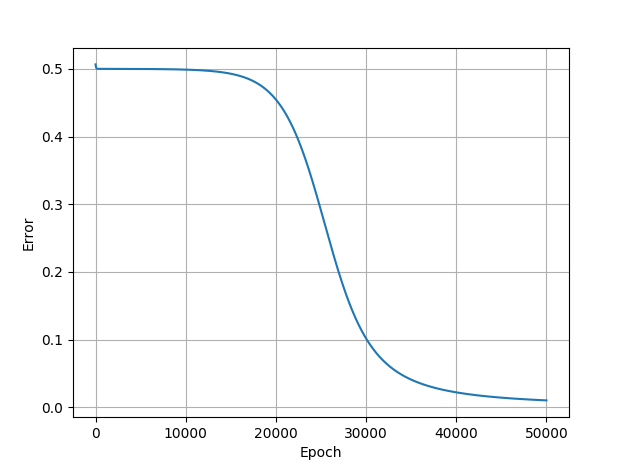
\includegraphics[width=\textwidth]{basic-error.png}
\caption{The mean square error of the basic neural network implementation over epochs}
\end{figure}
\clearpage

\subsubsection{Change in weights over 3 epochs}
The following table show cases how the values of each of the 2 weight matricies and 2 bias vectors change over each epoch.

\begin{center}
\begin{tabular}{|l|l|l|l|}
	\hline
	\textbf{Weights} & \textbf{Epoch 1} & \textbf{Epoch 2} & \textbf{Epoch 3}\\
	\hline
	$W_1$ &
$\begin{bmatrix}
0.09999288 & 0.19998892 \\
0.09998922 & 0.09999857 \\
\end{bmatrix}$  & 
$\begin{bmatrix}
0.09998587 & 0.19997799 \\
0.09997859 & 0.09999736 \\
\end{bmatrix}$ &
$\begin{bmatrix}
0.09997899 & 0.19996722 \\
0.09996813 & 0.09999637 \\
\end{bmatrix}$ \\
	\hline
	$W_2$ & 
$\begin{bmatrix}
0.09930886 & 0.09917138 \\
0.09930571 & 0.19916741 \\
\end{bmatrix}$  & 
$\begin{bmatrix}
0.09862415 & 0.09835049 \\
0.09861788 & 0.19834262 \\
\end{bmatrix}$ &
$\begin{bmatrix}
0.09794581 & 0.09753728 \\
0.09793647 & 0.19752554 \\
\end{bmatrix}$ \\
	\hline
	$b_1$ &
$\begin{bmatrix}
0.09992876 \\ 0.09988917 \\
\end{bmatrix}$  & 
$\begin{bmatrix}
0.09985872 \\ 0.0997799 \\
\end{bmatrix}$ &
$\begin{bmatrix}
0.099789887 \\ 0.09967217 \\
\end{bmatrix}$ \\
	\hline
	$b_2$ &
$\begin{bmatrix}
0.09872793 \\ 0.09841132 \\
\end{bmatrix}$  & 
$\begin{bmatrix}
0.09746791 \\ 0.09683713 \\
\end{bmatrix}$ &
$\begin{bmatrix}
0.09621986 \\ 0.09527734 \\
\end{bmatrix}$ \\
	\hline
\end{tabular}
\end{center}

From the above table it is apparent that the weights of the neuron to neuron synapses as well as the biases are changing, with all of the weights being decreased over time. The reason for weights decreasing is due to the optimal weight configuration values being less than the starting weights.\\ 
\clearpage

\subsubsection{Verifying Section 1}
The calculations for the partial derivatives found in section 1 will now be verified by printing each of the gradients from the python implementation.

\begin{figure}[!htb]
\centering
	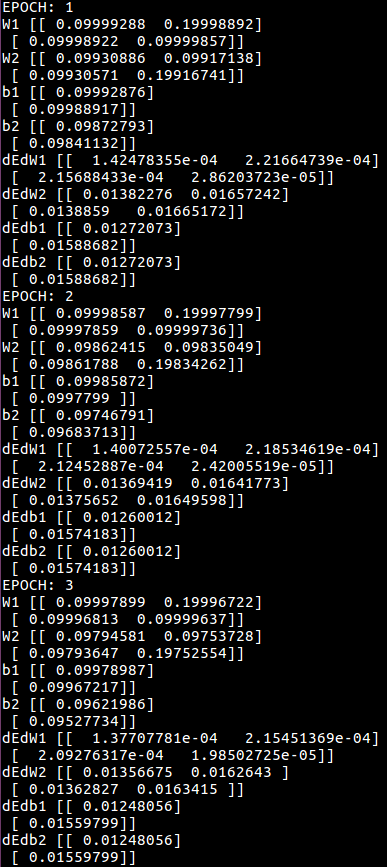
\includegraphics[scale=0.52]{verify.png}
\caption{Screenshot of output from the first 3 epochs of basic\_neural\_network.py}
\end{figure}
\clearpage

\subsection{MINST Neural Network}
Following on from the previous implementation of section 1, a neural network was implemented in python3 (see file $neural\_network.py$) that given a training data set was able to learn the details of hand written digits from 0-9. This neural network has 784 input, 30 hidden and 10 output neurons. The major difference between this implementation and the previous, is that this problem is of classification instead of regression and therefore a softmax function was used instead of a sigmoid for the final output $\hat{Y}$. As the softmax function returns the probability distribution of each exclusive class, it is possible to minimize the error by maximizing the probability of a class when its matching digit appears (e.g. when it is given an 8, the optimal output of the softmax function would be 1 for the 8 class and 0 for the other classes). The following sections explores the results of the neural network as the hyper parameters were altered.\\

\subsubsection{Initial Hyperparamater Results}
The initial hyperparamters of the neural network was stated to include a minibatch size of 20 samples, a learning rate of 3 and 30 epochs.

\begin{figure}[!htb]
\centering
	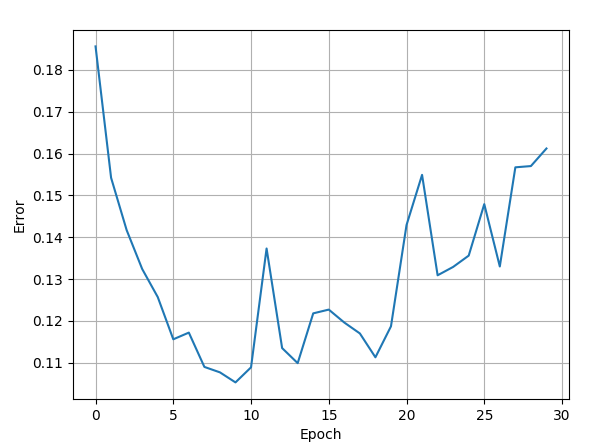
\includegraphics[scale=0.6]{lr3epoch30.png}
\caption{Error of the neural network on each epoch}
\end{figure}

The results shown above showcases underfitting between epoch 0 and epoch 9, in which the network still does not know enough and is `learning' the details of the classes. At epoch 9, the network is at its most accurate state guessing over 90\% of the test digits. After epoch 9, the network begins to overfit to the training data and learn the noise associated with it. Therefore, if these hyper parameters were to be used, the network should be trained until epoch 9 and then be stopped. This method was used to generate the predicted labels in files PredictTestY.csv.gz and PredictTestY2.csv.gz.

\subsubsection{Altering the Learning Rate}
The learning rate of a neural network is responsible for how big of a `step' the updated weights take in the direction of the global minima. The trade-offs associated with the learning rates are that if the step is too small, the network will take far too long to train, whilst having to large a learning rate will result in the algorithm `steping over' or `out' of the minima. These tradeoffs in the hyper-parameter are showcased below.

\begin{figure}[!htb]
\centering
	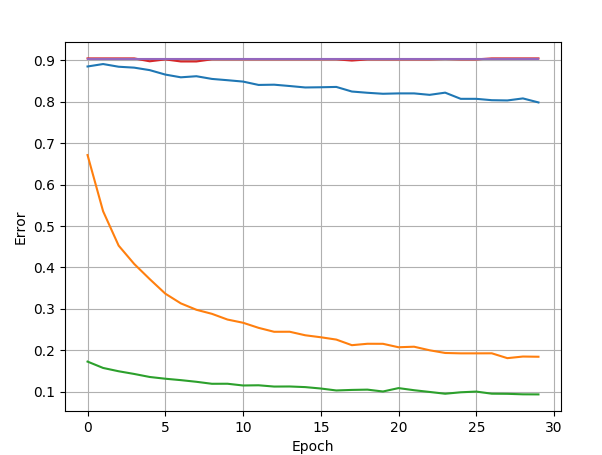
\includegraphics[scale=0.6]{all-lr.png}
\caption{Comparison of each neural networks error with differing learning rates}
\end{figure}

\begin{itemize}
\item $\eta = 100$ - Purple
\item $\eta = 10$ - Red
\item $\eta = 10$ - Blue
\item $\eta = 0.1$ - Yellow
\item $\eta = 0.001$ - Green
\end{itemize}

This comparison highlights the tradeoff mentioned above in which networks with large learning rates almost never converge to an error of near 0 as they are taking far to large a stride back and forth and how as the learning rate becomes more sensible, the network can take its time and eventually find and travel towards the global minima.

\subsubsection{Altering the Minibatch Size}
The size of the minibatch is similar to previous remarks as they both ends (small or large), both have pros and cons. Online learning (minibatchsize of 1) is known to be faster but does not always learn correctly as certain steps to the global minima are `undone' by others. Large minibatch sizes are slower to compute but yield lower error levels as a `compromise' is made between each of the gradients in which direction to move in.

\begin{figure}[!htb]
\centering
	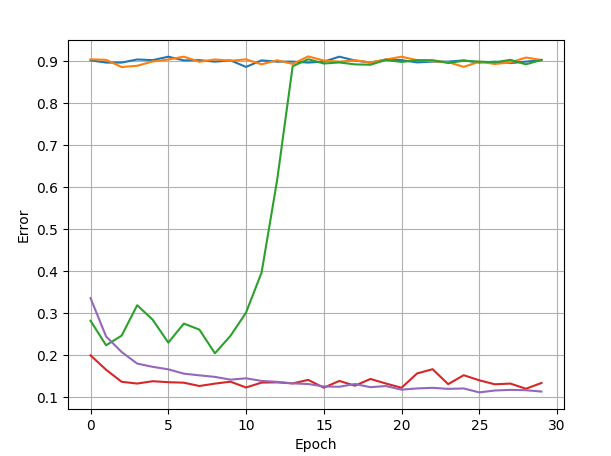
\includegraphics[scale=0.6]{all-mbs.png}
\caption{Comparison of each neural networks error with differing minibatch sizes}
\end{figure}

\begin{itemize}
\item 100 = purple
\item 20 = red
\item 10 = green
\item 5 = yellow
\item 1 = blue
\end{itemize}

\subsubsection{Altering Additional Hyperparameters}
Learning rates and minibatch sizes are not the only hyper-parameters that can be tweaked and adjusted to improve performance for a particular problem. For example the number of hidden layers in a network can easily be adjusted to try and improve performance.

\begin{figure}[!htb]
\centering
	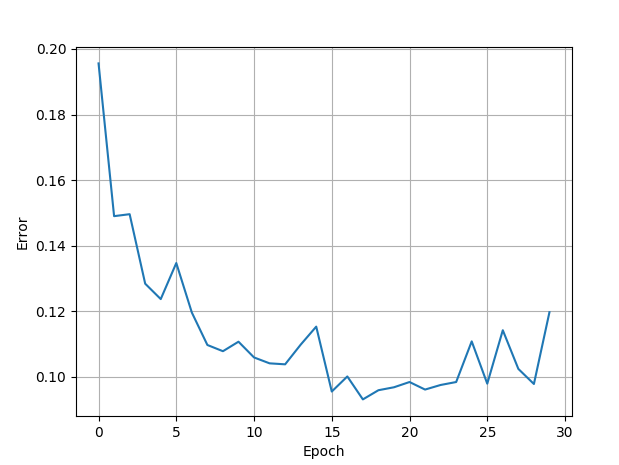
\includegraphics[scale=0.6]{hyper.png}
\caption{The neural network from section 2.2.1 but with hidden layer set to 35 neurons}
\end{figure}

As shown above, the network configuration from section 2.2.1 can be slightly changed to include 35 hidden neurons and further decrease the error from 0.09 to 0.05 (at both of their best epochs). 
\end{document}
